\chapter{Γραμμικός Προγραμματισμός}\label{ch:lp}
Ο στόχος του γραμμικού προγραμματισμού ,σύμφωνα με \cite{chong2010}, είναι να
προσδιορίσει τις τιμές των μεταβλητών που μεγιστοποιούν ή ελαχιστοποιούν μια γραμμική
αντικειμενική συνάρτηση, όπου οι μεταβλητές υπόκεινται σε κάποιους γραμμικούς περιορισμούς.
Το πρόβλημα του γραμμικού προγραμματισμού είναι μία ειδική κατηγορία ενός γενικού
προβλήματος βελτιστοποίησης με περιορισμούς. Στη γενική περίπτωση, ο στόχος είναι να βρούμε
ένα σημείο που ελαχιστοποιεί την αντικειμενική συνάρτηση και ταυτόχρονα ικανοποιεί τους περιορισμούς.
Οποιοδήποτε σημείο ικανοποιεί τους περιορισμούς ονομάζεται εφικτό σημείο. Στο πρόβλημα του γραμμικού
προγραμματισμού, η αντικειμενική συνάρτηση είναι γραμμική και το σύνολο των εφικτών σημείων καθορίζεται
από γραμμικές σχέσεις ισότητας και/ή ανισότητας.

Οι μέθοδοι για τη λύση προβλημάτων γραμμικού προγραμματισμού παρέχουν τη
δυνατότητα της επιλογής του καλύτερου εφικτού σημείου ανάμεσα στα πολλά εφικτά
σημεία. Γενικά, τα προβλήματα γραμμικού προγραμματισμού έχουν πολύ μεγάλο
μέγεθος, επομένως είναι απαραίτητοι αποδοτικοί μέθοδοι επίλυσης αυτών, που
πρωτοεμφανίστηκαν τέλη της δεκαετίας του 1930. Συγκεκριμένα το 1939, ο
\tl{Kantorovich} \cite{kantorovich1939}, παρουσίασε διάφορες λύσεις σε
προβλήματα σχετικά με το σχεδιασμό παραγωγής και μεταφορών. Κατά τη διάρκεια του
Δεύτερου Παγκοσμίου Πολέμου, ο \tl{Koopmans} \cite{koopmans1949} συνεισέφερε
σημαντικά στη λύση προβλημάτων μεταφοράς. Μάλιστα, και στους δύο προαναφερθέντες
απονεμήθηκε το Νόμπελ Οικονομίας το 1975 για τη συνεισφορά τους στη βέλτιστη κατανομή
πόρων. Το 1947, ο \tl{Dantzig} \cite{dantzig1963} ανέπτυξε μία καινούργια μέθοδο λύσης
γραμμικών προγραμμάτων, γνωστή ως μέθοδος \tl{simplex}. Η μέθοδος αυτή είναι αποδοτική, παρέχει
μία κομψή λύση για το πρόβλημα και χρησιμοποιείται ευρέως ως και σήμερα για τα προβλήματα
του γραμμικού προγραμματισμού. Παρόλο αυτά, ο αριθμός των βημάτων, και ως εκ
τούτου ο συνολικός χρόνος, για την εύρεση λύσης αυξάνει εκθετικά με το μέγεθος των μεταβλητών.
Αυτό οδήγησε στο ενδιαφέρον για τη σχεδίαση αλγορίθμων που θα λύνουν γραμμικά προγράμματα με
πολυωνυμική πολυπλοκότητα, δηλαδή αλγόριθμοι που θα βρίσκουν τη βέλτιστη λύση σε χρόνο που θα
εξαρτάται πολυωνυμικά με τον αριθμό των μεταβλητών. Ο \tl{Khachiyan} το 1979
\cite{khachiyan1979}, ήταν ο πρώτος που ανέπτυξε έναν τέτοιο αλγόριθμο, ωστόσο έλαβε
περισσότερο θεωρητικό παρά πρακτικό ενδιαφέρον. Το 1984, ο \tl{Karmarkar}
\cite{karmarkar1984} πρότεινε ένα νέο αλγόριθμο γραμμικού προγραμματισμού με
πολυωνυμική πολυπλοκότητα, που φαίνεται να λύνει προβλήματα αρκετά πιο αποδοτικά
από ότι η μέθοδος \tl{simplex}. Η δουλεία του \tl{Karmarkar} οδήγησε σε άλλες μεθόδους,
που δε βασίζονται στη μέθοδο \tl{simplex}, γνωστές ως μέθοδοι εσωτερικού σημείου
(\tl{interior-point}).

Ένα τυπικό γραμμικό πρόγραμμα βελτιστοποίησης είναι της μορφής
\begin{equation}\label{eq:lp_min}
    \begin{aligned}
        & {\text{\tl{minimize}}}
        & & \vc{c}^T \vc{x} \\
        & \text{\tl{subject to}}
        & & \mt{A} \vc{x} = \vc{b} \\
        &&& \vc{x} \ge \vc{0},
    \end{aligned}
\end{equation}
όπου $\vc{c} \in \mathbb{R}^n$, $\vc{b} \in \mathbb{R}^m$, και
$\mt{A} \in \mathbb{R}^{m \times n}$. Ο περιορισμός ανισότητας $\vc{x} \ge \vc{0}$
για τις μεταβλητές σημαίνει ότι κάθε συνιστώσα του διανύσματος $\vc{x}$
είναι μη αρνητική. Πολλές παραλλαγές του παραπάνω προβλήματος είναι δυνατές,
όπως για παράδειγμα, αντί για ελαχιστοποίηση της αντικειμενικής συνάρτησης να ζητούμε
τη μεγιστοποίηση αυτής. Επίσης, οι περιορισμοί θα μπορούσαν αντί ισότητα, να είχαν
τη μορφή ανισότητας, όπως $\mt{A}\vc{x} \ge \vc{b}$, ή $\mt{A}\vc{x} \le \vc{b}$.
Αναφερόμαστε σε αυτές τις παραλλαγές ως γραμμικό πρόγραμμα, καθώς είναι δυνατόν να γραφτούν στην παραπάνω μορφή.

Κάθε γραμμικό πρόγραμμα ικανοποιεί έμμεσα κάποιες υποθέσεις, όπως περιγράφονται
στο \cite{hillier1985}. Η \textbf{αναλογικότητα} (\tl{proportionality}) αναφέρεται σε
ξεχωριστές δραστηριότητες, που εξετάζονται ανεξάρτητα από τις υπόλοιπες.
Ας υποθέσουμε ότι από τις $n$ δραστηριότητες μόνο μία υλοποιείται και
ας την ονομάσουμε $k$,  έτσι ώστε, $x_j = 0$, για $j = 1, ..., n$, εκτός
από $j = k$. Σύμφωνα με αυτή την υπόθεση το μέτρο αποτελεσματικότητας
είναι ίσο με $c_k x_k$ και η χρησιμοποίηση κάθε πόρου $i$ είναι ίση
με $a_{ik}x_k$. Αυτό σημαίνει ότι οι δύο ποσότητες είναι ευθέως ανάλογες
προς το επίπεδο της $k$ δραστηριότητας. Ακόμη σημαίνει ότι δεν υπάρχουν
αρχικές επιβαρύνσεις με την έναρξη της δραστηριότητας και ότι η αναλογικότητα
ισχύει για όλα τα επίπεδα τιμών της δραστηριότητας.

Με την υπόθεση της αναλογικότητας δεν εξασφαλίζεται ότι η αντικειμενική συνάρτηση
και οι περιορισμοί είναι γραμμικές συναρτήσεις. Η \textbf{προσθετικότητα}
(\tl{additivity}) προϋποθέτει ότι δεν υπάρχουν αλληλεπιδράσεις μεταξύ των
δραστηριοτήτων. Για κάθε επίπεδο δραστηριοτήτων $(x_1,..., x_n)$ η
συνολική χρησιμοποίηση κάθε πόρου καθώς και το συνολικό μέτρο αποτελεσματικότητας
είναι ίσα με το άθροισμα των αντίστοιχων ποσοτήτων κάθε δραστηριότητας.

Μερικές φορές οι μεταβλητές αποφάσεων έχουν έννοια μόνο όταν παίρνουν
ακέραιες τιμές. Η λύση όμως που παίρνουμε από το γραμμικό προγραμματισμό
συχνά έχει μη ακέραιες τιμές. Με την υπόθεση της \textbf{διαιρετότητας}
(\tl{divisibility}) οι μονάδες δραστηριότητας μπορούν να διαιρεθούν σε
οποιοδήποτε κλασματικό επίπεδο, έτσι ώστε οι μη ακέραιες τιμές για τις μεταβλητές
αποφάσεων είναι επιτρεπτές.

\section{Επίλυση}
Στη συνέχεια θα παρουσιάσουμε κάποια παραδείγματα γραμμικού προγραμματισμού. Η
επίλυση αυτών έγινε με το λογισμικό \href{https://www.mathworks.com/products/matlab/}
{\tl{MATLAB}} και τη χρήση της βιβλιοθήκης βελτιστοποίησης (\tl{Optimization
Toolbox}) αυτού. Το \tl{MATLAB} δέχεται ένα γραμμικό πρόγραμμα στην παρακάτω μορφή
\begin{equation}\label{eq:lp_mat}
    \begin{aligned}
        & \underset{\vc{x}}{\text{\tl{minimize}}} & & \vc{f}^T \vc{x} \\
        & \text{\tl{subject to}} & & \mt{A} \vc{x} \leq \vc{b} \\
        &&& \mt{A}_{eq} \vc{x} = \vc{b}_{eq} \\
        &&& \vc{lb} \le \vc{x} \le \vc{ub}.
    \end{aligned}
\end{equation}
Στην παραπάνω σχέση, $\vc{f}$ είναι το διάνυσμα των συντελεστών της αντικειμενικής
συνάρτησης, $\mt{A}$ είναι το μητρώο των συντελεστών των ανισοτήτων και
$\vc{b}$ το αντίστοιχο διάνυσμα. Ακόμη, οι σχέσεις ισότητας περιγράφονται από το
μητρώο $\mt{A}_{eq}$ και το διάνυσμα $\vc{b}_{eq}$. Τέλος, $\vc{lb}$ και $\vc{ub}$ είναι
τα διανύσματα του κάτω και άνω ορίου του διανύσματος $\vc{x}$.

Η λύση γραμμικών προγραμμάτων γίνεται με τη συνάρτηση
\tl{\texttt{\textbf{linprog}}}. Η σύνταξή της είναι
\begin{otherlanguage}{english}
    \begin{center}
        \texttt{[x,fval,exitflag,output,lambda]=linprog(f,A,b,Aeq,beq,lb,ub,options)}
    \end{center}
\end{otherlanguage}
με απαραίτητα τα τρία πρώτα ορίσματα της συνάρτησης. Επιστρέφει τη βέλτιστη
λύση $\vc{x}$, την τιμή της αντικειμενικής συνάρτησης \tl{\texttt{fval}}, τη συνθήκη
εξόδου \tl{\texttt{exitflag}}, τη δομή (\tl{structure}) \tl{\texttt{output}}, σχετικά με
το τέλος του  προγράμματος και τους πολλαπλασιαστές \tl{Lagrange}
\tl{\texttt{lambda}}. Επίσης, από τη δομή \tl{\texttt{options}}, μπορούμε να ρυθμίσουμε
διάφορες παραμέτρους της διαδικασίας επίλυσης, όπως για παράδειγμα να επιλέξουμε
αλγόριθμο επίλυσης (\tl{interior-point, dual-simplex}), να θέσουμε ανοχές, δηλαδή το
κατά πόσο θα ικανοποιείται η αντικειμενική συνάρτηση, οι περιορισμοί, και άλλα πολλά.
Ο ενδιαφερόμενος παραπέμπεται στη βοήθεια του \tl{MATLAB}.

\subsection{Παράδειγμα 1}
Το πρώτο παράδειγμα προέρχεται από τη βοήθεια του \tl{MATLAB} και έχει
περιορισμούς ανισότητας, ισότητας καθώς και όρια στις μεταβλητές.
Η αντικειμενική συνάρτηση που θέλουμε να ελαχιστοποιήσουμε είναι
\begin{equation*}
    f(\vc{x}) = -x_1 - \frac{1}{3}x_2,
\end{equation*}
και οι σχέσεις ανισότητας που περιγράφουν το πρόβλημα είναι
\begin{align*}
    x_1 + x_2 &\leq 2 \\
    x_1 + \frac{1}{4}x_2 &\leq 1 \\
    x_1 - x_2 &\leq 2 \\
    -\frac{1}{4}x_1 - x_2 &\leq 1 \\
    -x_1 - x_2 &\leq -1 \\
    -x_1 + x_2 &\leq 2.
\end{align*}
Επίσης ισχύει ο περιορισμός ισότητας
\begin{equation*}
    x_1 + \frac{1}{4}x_2 = \frac{1}{2}
\end{equation*}
και τέλος έχουμε τα όρια
\begin{equation*}
    -1 \leq x_1 \leq 1.5, \qquad -0.5 \leq x_2 \leq 1.25.
\end{equation*}
Το παραπάνω πρόβλημα εύκολα γράφεται σε μητρωική μορφή και έτσι από τους περιορισμούς ανισότητας έχουμε
\begin{equation*}
    \mt{A} =
    \begin{bmatrix}
        1 & 1 \\
        1 & \frac{1}{4} \\
        1 & -1 \\
        -\frac{1}{4} & -1 \\
        -1 & -1 \\
        -1 & 1
    \end{bmatrix}, \qquad
    \vc{b} =
    \begin{bmatrix}
        2\\ 1\\ 2\\ 1\\ -1\\ 2
    \end{bmatrix}.
\end{equation*}
Ακόμη από τον περιορισμό ισότητας $\mt{A}_{eq} = \begin{bmatrix}1 & \frac{1}{4}\end{bmatrix}$,
$b_{eq} = \frac{1}{2}$, από τα κάτω και άνω όρια προκύπτει
$\vc{lb} = \begin{bmatrix}-1 & -0.5 \end{bmatrix}^T$, $\vc{ub} = \begin{bmatrix}1.5 & 1.25 \end{bmatrix}^T$
και τέλος από την αντικειμενική συνάρτηση έχουμε το διάνυσμα
$\vc{f} = \begin{bmatrix}-1 & -\frac{1}{3}\end{bmatrix}^T$. Λύνοντας το πρόβλημα,
βρίσκουμε ότι η βέλτιστη λύση είναι $\vc{x}^* = \begin{bmatrix} 0.1875 & -1.25 \end{bmatrix}^T$
και η αντίστοιχη τιμή της αντικειμενικής $f(\vc{x}^*) = -0.6042$. Παρακάτω παρατίθεται ο κώδικας
που χρησιμοποιήθηκε για να λυθεί το πρόβλημα.
\begin{otherlanguage}{english}
\lstinputlisting[language=Matlab]{src/lp1.m}
\end{otherlanguage}

\subsection{Παράδειγμα 2}
Το επόμενο παράδειγμα πρόκειται για πρόβλημα μεγιστοποίησης και καθότι πιο απλό,
είναι ιδιαίτερα χρήσιμο για να δούμε γεωμετρικά τη λύση του γραμμικού προγράμματος.
Το πρόβλημα είναι το εξής,
\begin{equation*}
    \begin{aligned}
        & \underset{\vc{x}}{\text{\tl{maximize}}} & & 4x + 3y \\
        & \text{\tl{subject to}} & & 2y \leq 25 - x \\
        &&& 4y \geq 2x - 8 \\
        &&& y \leq 2x - 5 \\
        &&& x \geq 0 \\
        &&& y \geq 2,
    \end{aligned}
\end{equation*}
ή στην ισοδύναμη συμπαγή μορφή
\begin{equation*}
    \begin{aligned}
        & \underset{\vc{x}}{\text{\tl{minimize}}} & & \vc{f}^T\vc{x} \\
        & \text{\tl{subject to}} & & \vc{A}\vc{x} \leq \vc{b},
    \end{aligned}
\end{equation*}
όπου $\vc{x} = \begin{bmatrix} x & y\end{bmatrix}^T$, $\vc{f} = \begin{bmatrix}-4 & -3\end{bmatrix}^T$ και
\begin{equation*}
    \mt{A} =
    \begin{bmatrix}
        1 & 2 \\
        2 & -4 \\
        -2 & 1 \\
        -1 & 0 \\
        0 & -1
    \end{bmatrix}, \qquad
    \vc{b} =
    \begin{bmatrix}
        25\\ 8\\ -5\\ 0\\ -2
    \end{bmatrix}.
\end{equation*}
Είναι προφανές ότι ένα πρόβλημα μεγιστοποίησης είναι το αντίθετο από ένα πρόβλημα ελαχιστοποίησης,
για αυτό μπορούμε εύκολα να γράψουμε το γραμμικό πρόγραμμα σε μορφή που
αναγνωρίζει το \tl{MATLAB}. Λύνοντας το πρόβλημα, βρίσκουμε ότι η βέλτιστη λύση
είναι $\vc{x}^* = \begin{bmatrix} 14.5 & 5.25 \end{bmatrix}^T$ και η αντίστοιχη τιμή
της αντικειμενικής $f(\vc{x}^*) = 73.75$. Παρακάτω παρατίθεται ο κώδικας που
χρησιμοποιήθηκε για να λυθεί το πρόβλημα.
\begin{otherlanguage}{english}
\lstinputlisting[language=Matlab]{src/lp2.m}
\end{otherlanguage}
Παρακάτω παρουσιάζεται η γραφική λύση του γραμμικού προγράμματος.
\begin{figure}[h]
    \centering
    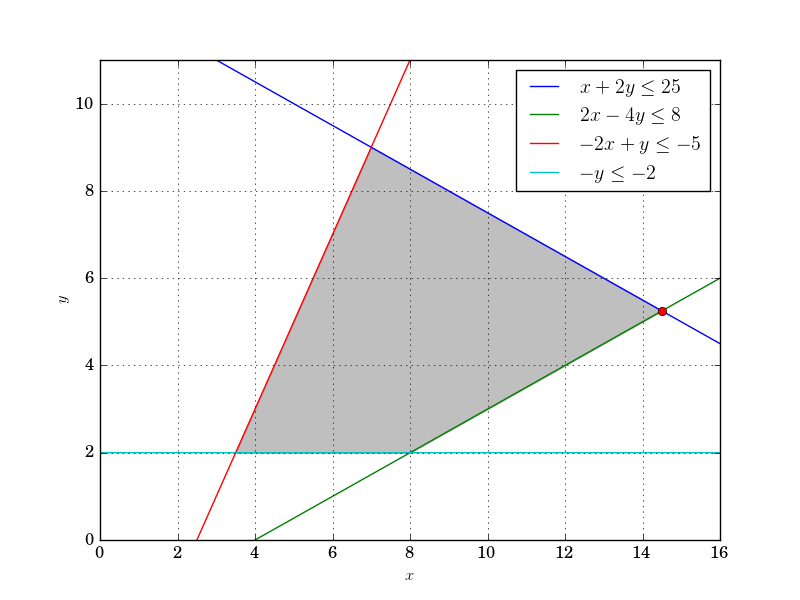
\includegraphics[width=\textwidth]{figures/lp2.png}
    \caption{Γραφική λύση του παραδείγματος 2
    του γραμμικού προγραμματισμού}\label{fig:lp2}
\end{figure}
Όπως φαίνεται από το σχήμα \ref{fig:lp2} οι περιορισμοί του προβλήματος δημιουργούν
ένα πολύγωνο, γκρι σκιαγράφηση, όπου είναι ο χώρος των δυνατών λύσεων. Τελικά από όλα
τα σημεία του πολυγώνου το βέλτιστο φαίνεται στο σχήμα με την κόκκινη κουκκίδα και είναι
αυτό που μεγιστοποιεί την αντικειμενική συνάρτηση.

\subsection{Παράδειγμα 3}
Τα δεδομένα του επόμενου παραδείγματος προέρχονται από
\href{http://pythonhosted.org/PuLP/CaseStudies/a_blending_problem.html}{εδώ}.
Σύμφωνα με το παράδειγμα πρόκειται για ένα πραγματικό πρόβλημα γραμμικού προγραμματισμού.
Μία εταιρία που φτιάχνει τροφές για γάτες, επιδιώκει το χαμηλότερο δυνατό κόστος καθώς
και την επίτευξη των διατροφικών στόχων που έχουν τεθεί. Οι στόχοι αυτοί για τα $100 g$
προϊόντος, είναι τουλάχιστον $8 g$ πρωτεΐνης και $6 g$ λιπαρών, αλλά όχι παραπάνω
από $2 g$ φυτικών ινών και $0.4 g$ αλατιού. Επιδιώκουν δηλαδή να βρουν τη σωστή
αναλογία των βασικών συστατικών που μπορούν να χρησιμοποιήσουν(τα βασικά συστατικά
είναι κοτόπουλο, βοδινό, αρνί, ρύζι, σιτάρι και τζελ), ούτως ώστε να ικανοποιηθούν
οι στόχοι που αναφέραμε. Τα κόστη ανά γραμμάριο του κοτόπουλου, του βοδινού και του
αρνιού είναι $0.013\$$, $0.008\$$ και $0.01\$$ αντίστοιχα, ενώ του ρυζιού, του
σιταριού και του τζελ $0.002\$$, $0.005\$$ και $0.001\$$ αντίστοιχα. Κάθε βασικό
συστατικό συνεισφέρει στο συνολικό βάρος πρωτεΐνης, λιπαρών, φυτικών ινών και αλατιού
στο τελικό προϊόν. Η συνεισφορά του καθενός (σε γραμμάρια) ανά γραμμάριο συστατικού
παρουσιάζονται στο παρακάτω πίνακα.
\begin{table}[h]
    \centering
    \begin{tabulary}{0.95\textwidth}{ | p{2cm} | C | C | C | C | }
        \hline
        {}        & Πρωτεΐνη & Λιπαρά & Φυτικές Ίνες & Αλάτι \\ \hline
        Κοτόπουλο      & $0.1$             & $0.08$                    & $0.001$                   & $0.002$ \\ \hline
        Χοιρινό      & $0.2$            & $0.1$                    & $0.005$                 & $0.005$ \\ \hline
        Αρνί      & $0.15$            & $0.11$                    & $0.003$                 & $0.007$ \\ \hline
        Ρύζι      & $0$             & $0.01$                    & $0.1$                  & $0.002$ \\ \hline
        Σιτάρι      & $0.04$            & $0.01$                    & $0.15$                 & $0.008$  \\ \hline
        Τζελ     & $0$             & $0$                    & $0$                  & $0$ \\ \hline
    \end{tabulary}
    \caption{Πίνακας Συστατικών}\label{table:lp3}
\end{table}
Αρχικά θα ορίσουμε ως μεταβλητές, το ποσοστό των συστατικών που μπορεί να
περιέχεται στη συσκευασία. Επειδή η συσκευασία είναι $100g$, τα ποσοστά
αυτά αντιπροσωπεύουν την ποσότητα των γραμμαρίων του κάθε συστατικού.
Ορίζουμε ως $x_1$ το ποσοστό του κοτόπουλου που περιέχεται στη
συσκευασία, $x_2$ το αντίστοιχο ποσοστό βοδινού, $x_3$ το ποσοστό
αρνιού, $x_4$ ρυζιού, $x_5$ φυτικών ινών και $x_6$ το ποσοστό
του τζελ. Στόχος είναι η μείωση του κόστους, και ορίζουμε ως
αντικειμενική συνάρτηση προς ελαχιστοποίηση
\begin{equation*}
    0.013x_1 + 0.008x_2 + 0.01x_3 + 0.002x_4 + 0.005x_5 + 0.001x_6,
\end{equation*}
σε δολάρια. Οι περιορισμοί του προβλήματος, έχουν περιγραφεί
παραπάνω και μπορούν να γραφτούν
\begin{align*}
    0.1x_1 + 0.2x_2 + 0.15x_3 + 0.04x_5 &\geq 8 \\
    0.08x_1 + 0.1x_2 + 0.11x_3 + 0.01x_4 + 0.01x_5 &\geq 6 \\
    0.001x_1 + 0.005x_2 + 0.003x_3 + 0.1x_4 + 0.15x_5 &\leq 2 \\
    0.002x_1 + 0.005x_2 + 0.007x_3 + 0.002x_4 + 0.008x_5 &\leq 2.
\end{align*}
Επίσης, έχουμε έναν προφανή περιορισμό ισότητας, ότι το
άθροισμα των συστατικών πρέπει να ισούται με όλη τη συσκευασία, δηλαδή
\begin{equation*}
    x_1 + x_2 + x_3 + x_4 + x_5 + x_6 = 100.
\end{equation*}
Τέλος, για κάθε ένα συστατικό $i$, έχουμε ένα κάτω και ένα
άνω όριο όπως φαίνεται στην παρακάτω σχέση
\begin{equation*}
    0 \leq x_i \leq 100.
\end{equation*}
Το παραπάνω πρόβλημα εύκολα γράφεται σε μητρωική μορφή και
έτσι από τους περιορισμούς ανισότητας έχουμε
\begin{equation*}
    \mt{A} =
    \begin{bmatrix}
        -0.1 & -0.2 & -0.15 & 0 & -0.04 & 0\\
        -0.08 & -0.1 & -0.11 & -0.01 & -0.01 & 0\\
        0.001 & 0.005 & 0.003 & 0.1 & 0.15 & 0\\
        0.002 & 0.005 & 0.007 & 0.002 & 0.008 & 0
    \end{bmatrix}, \qquad
    \vc{b} =
    \begin{bmatrix}
        -8\\ -6\\ 2\\ 0.4
    \end{bmatrix}.
\end{equation*}
Ακόμη από τον περιορισμό ισότητας $\mt{A}_{eq} = \begin{bmatrix}1 & 1 & 1 & 1 & 1 & 1\end{bmatrix}$,
$b_{eq} = 100$, από τα κάτω και άνω όρια προκύπτει
$\vc{lb} = \vc{0}_{6\times 1}^T$, $\vc{ub} = 100\vc{I}_{6 \times 1}^T$
και τέλος από την αντικειμενική συνάρτηση έχουμε το διάνυσμα
$\vc{f} = \begin{bmatrix}0.013 & 0.008 & 0.01 & 0.002 & 0.005 & 0.001\end{bmatrix}^T$.
Λύνοντας το πρόβλημα, βρίσκουμε ότι η βέλτιστη λύση είναι
$\vc{x}^* = \begin{bmatrix} 0 & 60 & 0 & 0 & 0 & 40\end{bmatrix}^T$,
δηλαδή $60\%$ βοδινό κρέας και $40\%$ τζελ, και η αντίστοιχη τιμή της
αντικειμενικής $f(\vc{x}^*) = 0.52$ δολάρια ανά συσκευασία.
Παρακάτω παρατίθεται ο κώδικας που χρησιμοποιήθηκε για να λυθεί το πρόβλημα.
\begin{otherlanguage}{english}
\lstinputlisting[language=Matlab]{src/lp3.m}
\end{otherlanguage}
